%!TEX root = ../main.tex
\setcounter{chapter}{7}
\setcounter{section}{1}
\section{Dynamic Analysis of Discrete Systems}
\vspace{-8pt} \hrule \hrule \hrule \hrule \hrule  \vspace{12pt}
	\begin{enumerate}
		\setcounter{enumi}{3}
\item See Fig. 8.4, and it shows the mapping of lines of constant damping $\zeta$ and natural frequency $\omega_n$ from $s$-plane to the upper half of the $z$-plane, using $z = e^{sT}$. 
		\begin{figure}[h]
		    \centering
			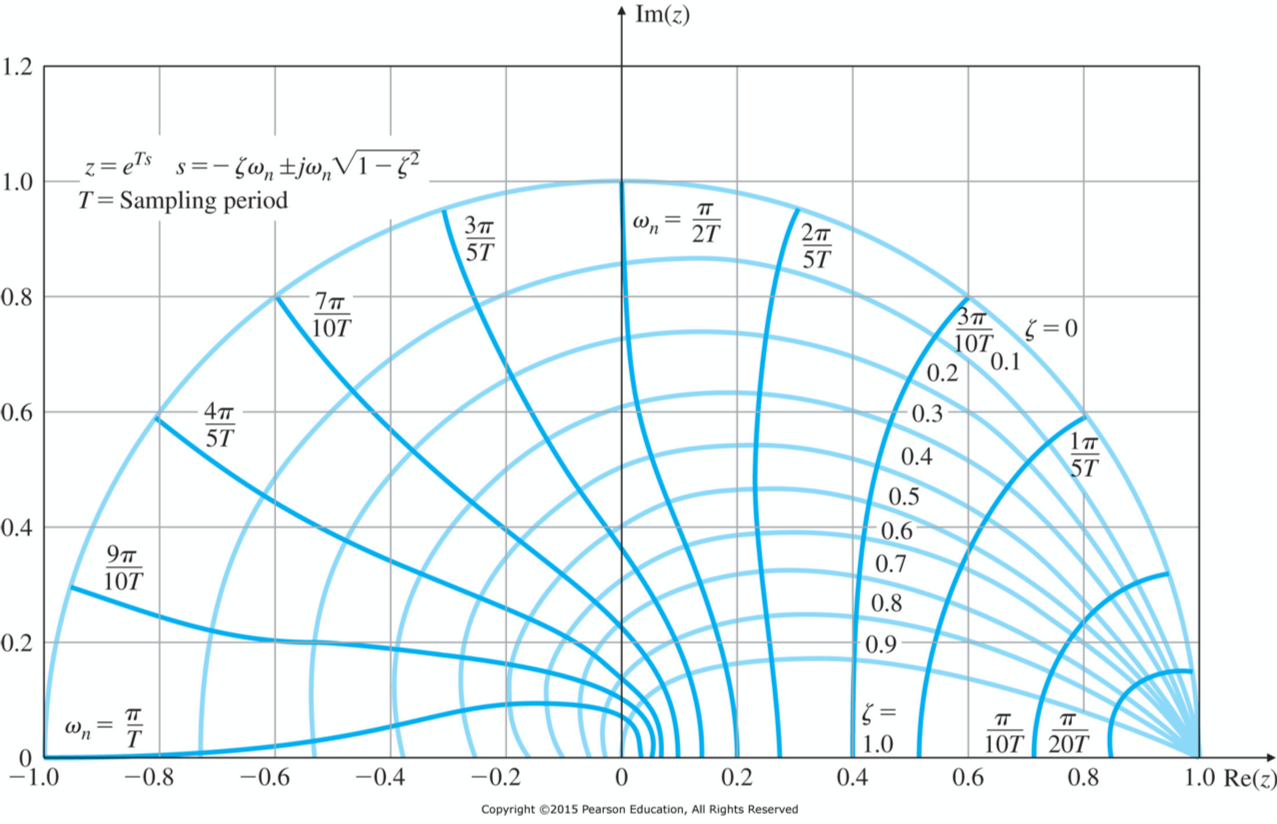
\includegraphics[width=10cm]{./FIG_Franklin/fig8-4.png}
		\end{figure}
		\begin{enumerate}
			\item The stability boundary $s= 0 \pm j\omega$ becomes the unit circle $|z| =1$ in the $z$-plane; inside the unit circle is stable, outside is unstable\\
			s-plane에서의 stability boundary는 imaginary축 $s = \pm j\omega$ 인데 z-plane에서의 stability boundary는 unit circle $|z|=e^{sT}|_{s=\pm j \omega }= 1 $이 된다.
			\item The small vicinity around $z=+1$ in the $z$-plane is essentially identical to the vicinity around the origin $s=0$, in the $s$-plane.\\
			z-plane 에서의 $z=1$근방은 s-plane에서의 $s=0$ 근방과 같다.
			\item The $z$-plane locations give response information normalized to the sample rate rather than to time as in the $s$-plane. \\
			z-plane 에서의 response information은 s-plane에서와 같이 시간에 대한 정보가 아닌, sample rate로 normalized된 정보를 제공한다.
			\newpage
			\item The negative real $z$-axis always represents a frequency of $\omega_s/2$, where $\omega_s = 2\pi/T = $ circular sample rate in radians per second.\\
			 $\omega_s$가  $2\pi/T$ 일때 음의 $z$축은 $\omega_s/2$로 표현된다.
			\item Vertical lines in the left half of the $s$-plane (the constant real part of $s$) map into \emph{circles} within the unit circle of the $z$-plane \\
			s-plane에서의 좌반면은 z-plane에서의 unit circle 내부로 매핑된다.
			\item Horizontal lines in the $s$-plane (the constant imaginary part of $s$) map into \emph{radial lines} in the $z$-plane. \\
			s-plane에서의 수평선은 z-plane에서의 radial line들로 매핑된다.
			\item Frequencies greater than $\omega_s/2$, called the Nyquist frequency, appear in the $z$-plane on the top of corresponding lower frequencies because of the circular characteristics of $e^{sT}$. This overlap is called \emph{aliasing} or folding.  
		\end{enumerate} 
		\item As a result, it is necessary to sample at least twice as fast as a signal's highest frequency component in order to represent that signal with the samples. 
		\item The figure sketches time responses that would result from poles at the indicated locations.
		\begin{figure}[h]
			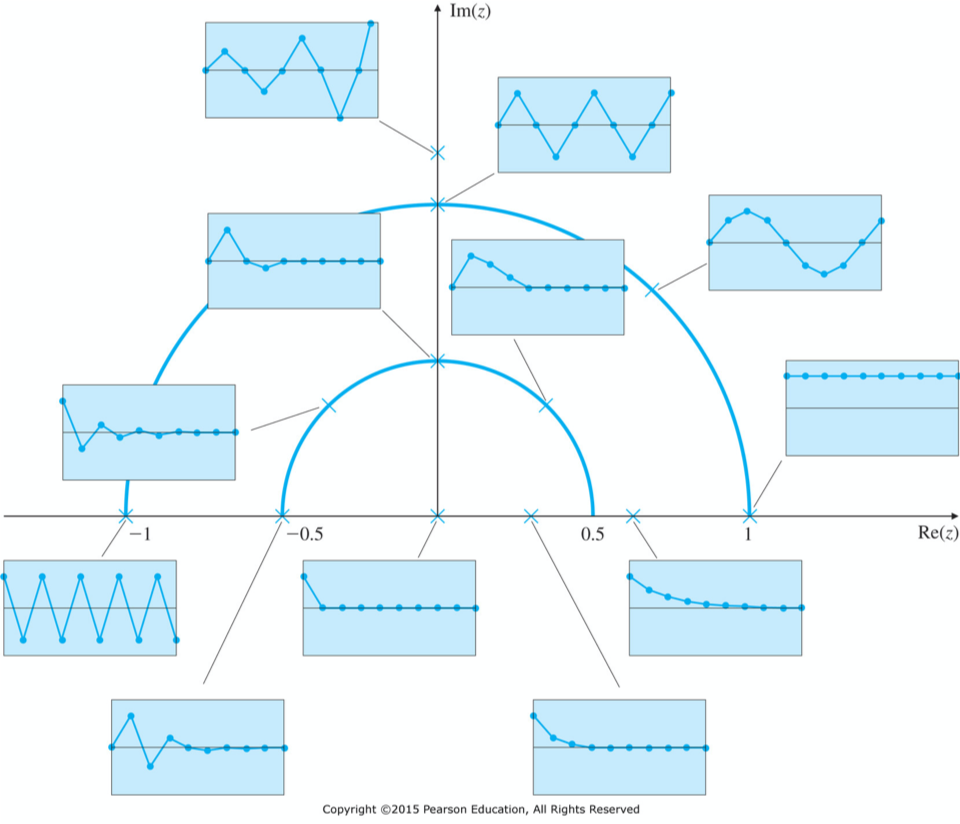
\includegraphics[width=14cm]{./FIG_Franklin/fig8-5.png}
		\end{figure}
	\end{enumerate}